	\chapter{Hardwaregrundlagen}
		\section{Flynn's Taxonomy}
		Aus Wikipedia \autocite{wikiFT}:
		
		Die Flynn’sche Taxonomie wurde 1966 von Michael J. Flynn publiziert und beschreibt eine grobe Unterteilung von Rechnerarchitekturen basierend auf der Anzahl der Befehls- (instruction streams) und Datenströme (data streams). Die Klassifikation teilt im Wesentlichen vier Bereiche ein:
		
		\begin{itemize}
		\item \textbf{Single Instruction, Single Data (SISD)}\\ Unter SISD-Rechnern versteht man traditionelle Einkernprozessor-Rechner, die ihre Aufgaben sequentiell abarbeiten. SISD-Rechner sind z. B. Personal-Computer (PCs) oder Workstations, welche nach der Von-Neumann- oder der Harvard-Architektur aufgebaut sind. Bei ersterer wird für Befehle und Daten die gleiche Speicheranbindung verwendet, bei letzterer sind sie getrennt. 
		
		\item \textbf{Single Instruction, Multiple Data (SIMD)}\\ Eine Architektur von Großrechnern beziehungsweise Supercomputern. SIMD-Computer, auch bekannt als Array-Prozessoren oder Vektorprozessor, dienen der schnellen Ausführung gleichartiger Rechenoperationen auf mehrere gleichzeitig eintreffende oder zur Verfügung stehende Eingangsdatenströme und werden vorwiegend in der Verarbeitung von Bild-, Ton- und Videodaten eingesetzt.

Dies ist sinnvoll, weil in diesen Bereichen die zu verarbeitenden Daten meist hochgradig parallelisierbar sind. So sind z. B. bei einem Videoschnitt die Operationen für die vielen einzelnen Bildpunkte identisch. Theoretisch optimal wäre hier die Ausführung durch einen einzigen, auf alle Punkte anzuwendenden Befehl.

Des Weiteren sind im Multimedia- und Kommunikationsbereich erforderliche Operationen häufig keine einfachen, einzelnen Operationen, sondern eher umfangreichere Befehlsketten. Das Einblenden eines Bildes vor einem Hintergrund ist beispielsweise ein komplexer Vorgang aus Maskenbildung mittels XOR, Vorbereitung des Hintergrundes mittels AND und NOT, sowie der Überlagerung der Teilbilder durch OR. Dieser Anforderung wird durch die Bereitstellung neuer komplexer Befehle entsprochen. So vereinigt z. B. der MMX-Befehl PANDN eine Invertierung und Und-Verknüpfung der Form x = y AND (NOT x).

Viele moderne Prozessorarchitekturen (wie PowerPC und x86) beinhalten inzwischen SIMD-Erweiterungen, das heißt spezielle zusätzliche Befehlssätze, die mit einem Befehlsaufruf gleichzeitig mehrere gleichartige Datensätze verarbeiten.

Allerdings muss man zwischen Befehlen unterscheiden, die lediglich gleichartige Rechenoperationen ausführen und anderen, die bis in den Bereich der DSP-Funktionalität hineinreichen (beispielsweise ist AltiVec in dieser Hinsicht wesentlich leistungsfähiger als 3DNow). 

    \item \textbf{Multiple Instruction, Single Data (MISD)}\\ Eine Architektur von Großrechnern bzw. Supercomputern. Die Zuordnung von Systemen zu dieser Klasse ist schwierig, sie ist deshalb umstritten. Viele sind der Meinung, dass es solche Systeme eigentlich nicht geben dürfte. Man kann aber fehlertolerante Systeme, die redundante Berechnungen ausführen, in diese Klasse einordnen. Ein Beispiel für dieses Prozessorsystem ist ein Schachcomputer.

Eine Umsetzung ist das Makropipelining, bei dem mehrere Recheneinheiten hintereinander geschaltet sind. Eine weitere sind redundante Datenströme zur Fehlererkennung bzw. -korrektur. 

    \item \textbf{Multiple Instruction, Multiple Data (MIMD)}\\ Eine Architektur von Großrechnern bzw. Supercomputern. MIMD-Computer führen gleichzeitig verschiedene Operationen auf verschieden gearteten Eingangsdatenströmen durch, wobei die Verteilung der Aufgaben an die zur Verfügung stehenden Ressourcen, meistens durch einen oder mehrere Prozessoren des Prozessorverbandes, selbst zur Laufzeit durchgeführt wird. Jeder Prozessor hat Zugriff auf die Daten anderer Prozessoren.

Man unterscheidet eng gekoppelte Systeme und lose gekoppelte Systeme. Eng gekoppelte Systeme sind Mehrprozessorsysteme, während lose gekoppelte Systeme Multicomputersysteme sind.

Multiprozessorsysteme teilen sich den vorhandenen Speicher und sind somit also ein shared-Memory System. Diese shared-Memory Systeme lassen sich weiter in UMA (uniform memory access), NUMA (non-uniform memory access) und COMA (cache-only memory access) unterteilen.

Man versucht bei MIMD eine Problemstellung durch die Lösung von Teilproblemen in den Griff zu bekommen. Dabei entsteht wiederum das Problem, dass verschiedene Teilstränge des Problems miteinander synchronisiert werden müssen.

Ein Beispiel in diesem Falle wäre das UNIX-Kommando make. Hier können auch mit mehreren Prozessoren mehrere zusammengehörige Programmcodes gleichzeitig in Maschinensprache übersetzt werden. 
        \end{itemize}
        
        \section{Aufbau einer Grafikkarte}
        Auch wenn das Moor'sche Gesetz noch ansatzweise erfüllt ist, stagniert die Leistung von einzelnen Prozessoren seit Jahren (Abb. \ref{2:hard}). Folglich versucht man viele Prozessoren zu einem großen Verbund zusammen zu schalten.
        
        \begin{figure}[h]
			\centering
    		    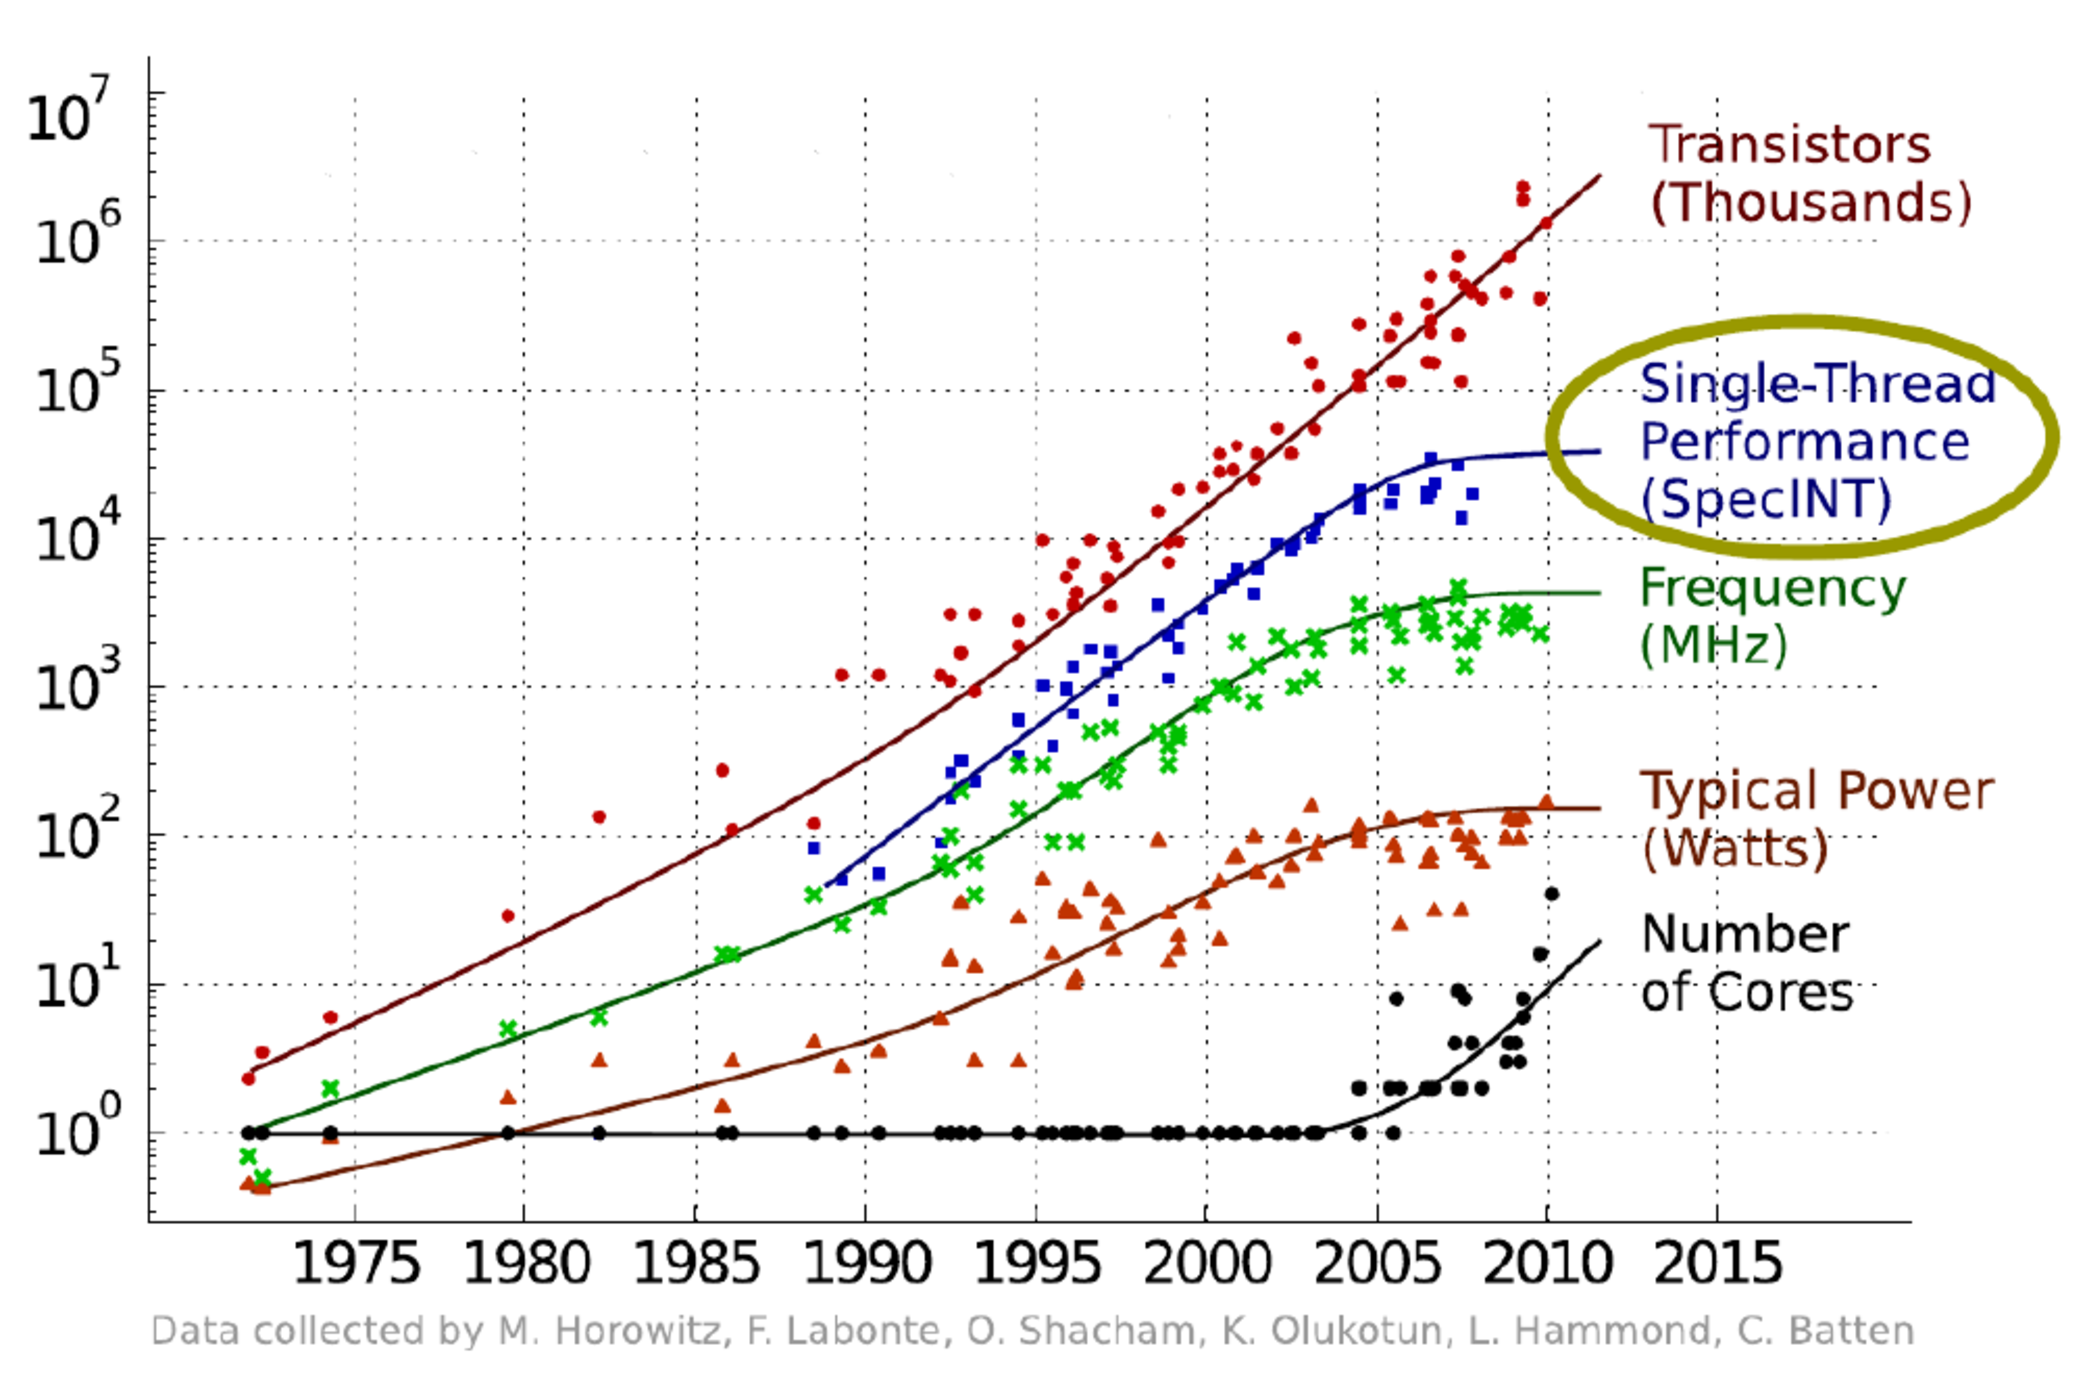
\includegraphics[width=0.8\textwidth]{chapter2/pictures/perf.pdf}
    		    \caption[Hardware]{Entwicklung der Hardware}
    		    \label{2:hard}
		\end{figure}
		
		\newpage

		Die Idee: nutze Grafikkarten als co-Prozessoren. Eine Grafikkarte besteht aus mehreren Teilen (Abb. \ref{2:graka}):
		\begin{itemize}
			\item \textbf{Bus Interface}: steuert den Datenfluss von der \Gls{PCIe}-Schnittstelle, Instruktionen werden an die GPU weitergeleitet, Speicherallozierungen an den Speichercontroller
			\item \textbf{Speichercontroller}: ein kleiner Mikroprozessor, der Speicher alloziert
			\item \textbf{Speicher}: beinhaltet den globalen und Texturspeicher. Die interne Speicherbandbreite liegt heutzutage bei bis zu 1TB/s (HBM2).
			\item \textbf{GPU}: das Herzstück der Grafikkarte. Ursprünglich war die einzige Aufgabe, der CPU 3d-Berechnungen für Texturen abzunehmen. Es existieren Grafikkarten mit zwei GPUs.
			\item \textbf{Video-Out-Controller}: wandelt die Berechnungen der GPU in Signale für die Videoausgänge um. Ein DAC Wandler wird nur für den VGA-Ausgang benötigt und existiert auf modernen Karten nicht mehr. 			
		\end{itemize}
		
		\begin{figure}[h]
			\centering
    		    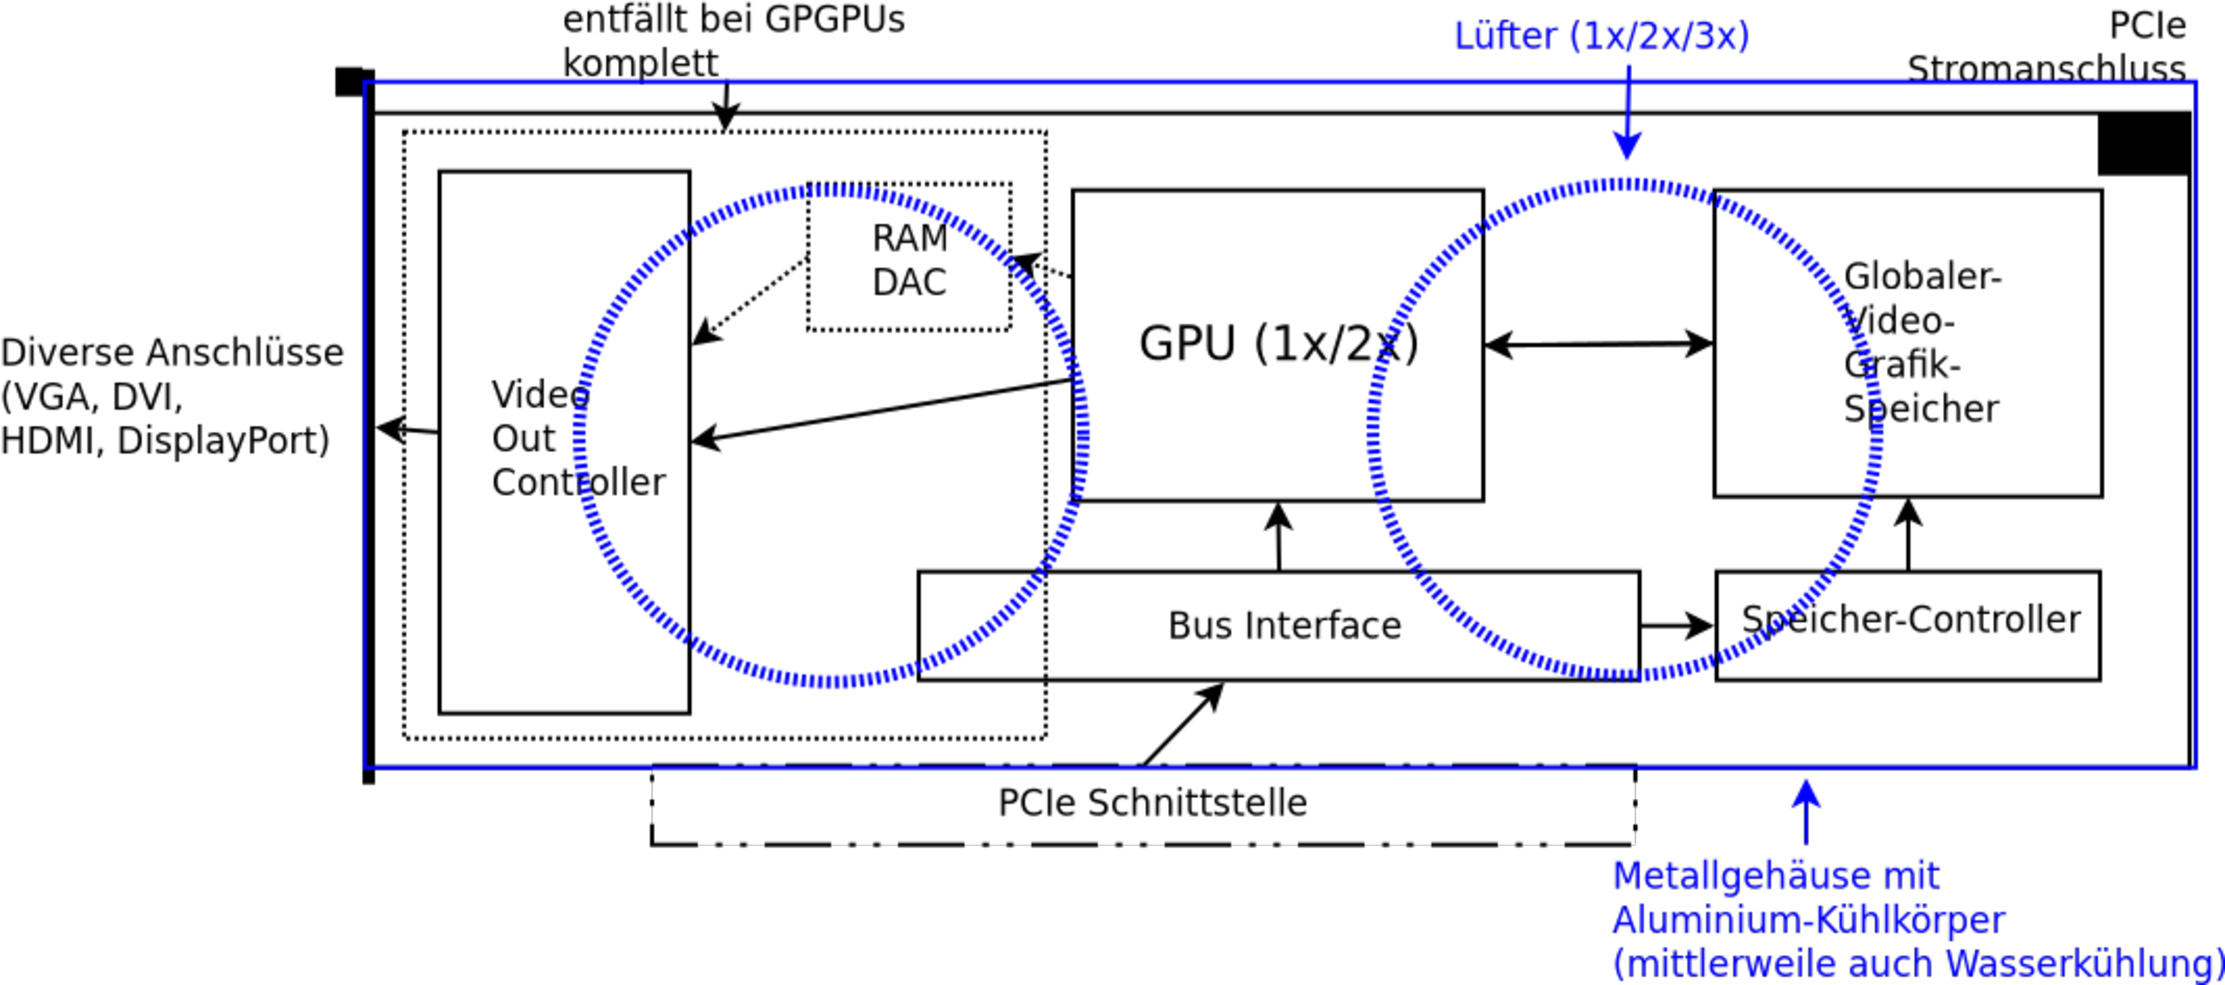
\includegraphics[width=\textwidth]{chapter2/pictures/gpu.pdf}
    		    \caption[Grafikkarte]{Teile einer Grafikkarte}
    		    \label{2:graka}
		\end{figure}
		
		Auf jeder GPU sitzt ein passiv-Kühler sowie ein separater Lüfter. Abbildung \ref{2:gpucpu} zeigt eine Grafikkarte verbaut in einem gewöhnlichen Desktop Computer.
		
		\newpage
		
		\begin{figure}[h]
			\centering
    		    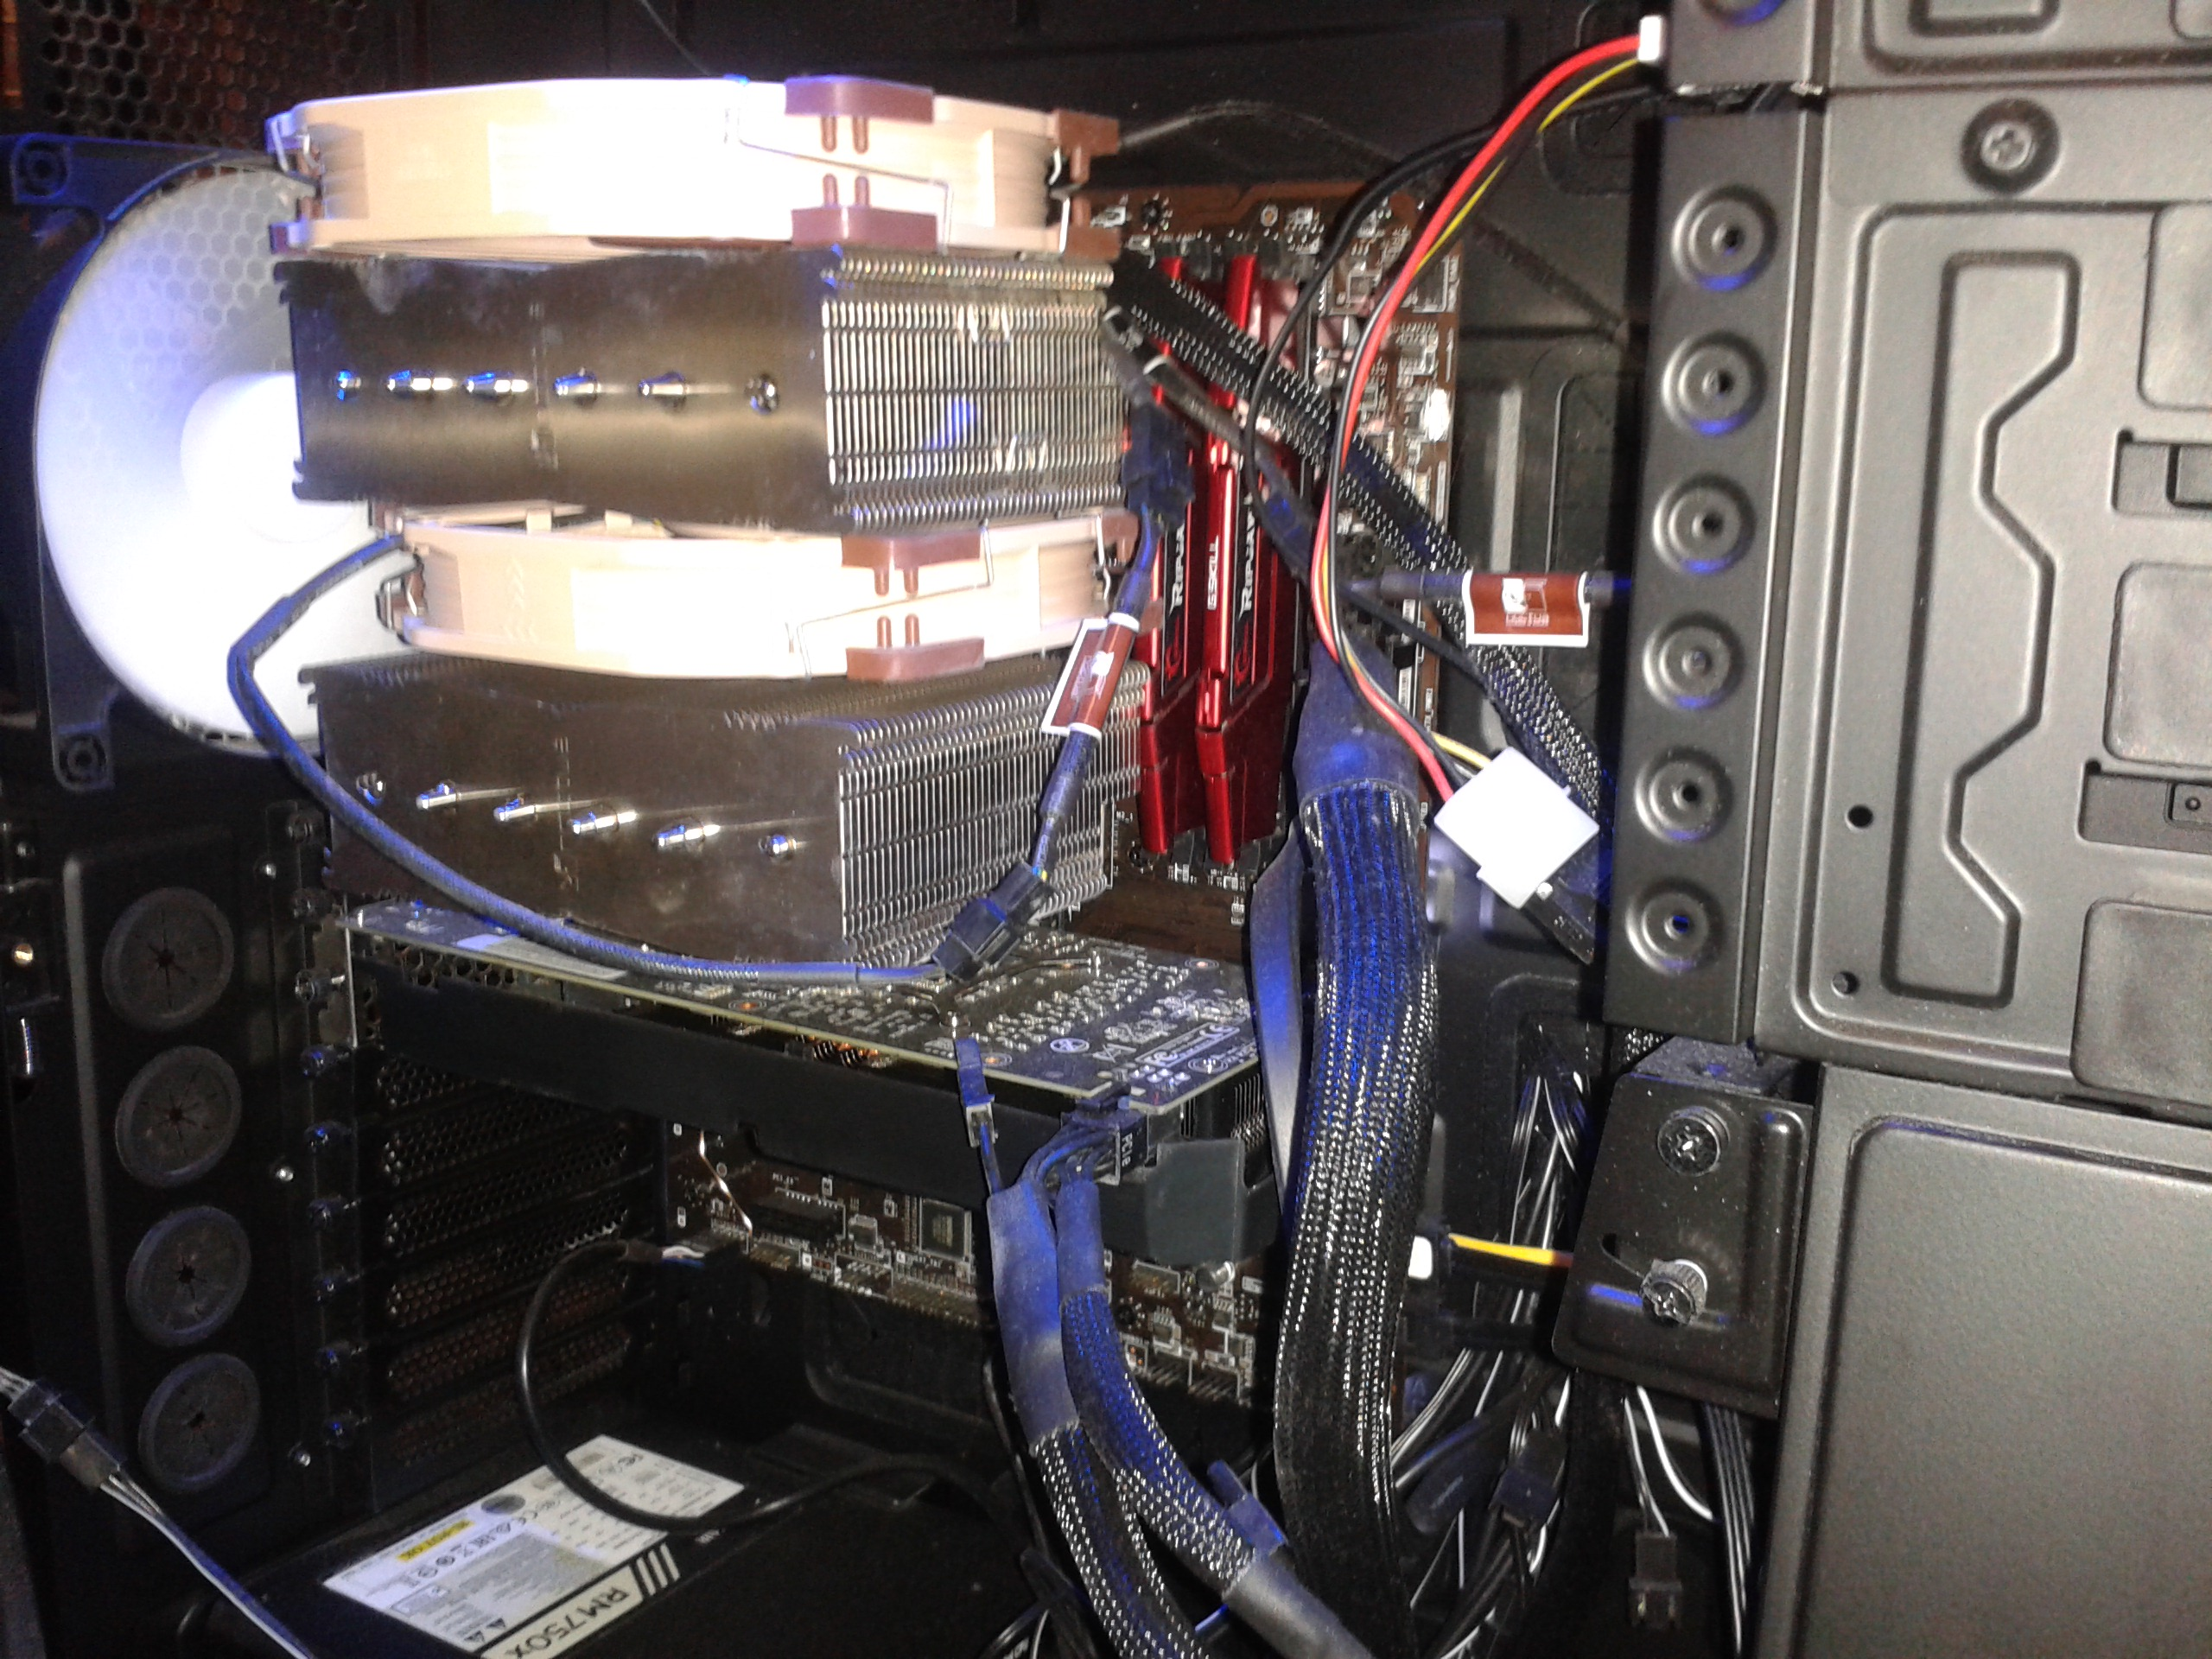
\includegraphics[height=0.6\textwidth]{chapter2/pictures/pc.pdf}
    		    \caption[Desktop PC]{Aufbau eines gewöhnlichen Desktop-Computers}
    		    \label{2:gpucpu}
		\end{figure}
		
		Datenverkehr zwischen CPU und GPU erfolgt meistens über \Gls{PCIe}x16 mit einer maximalen physikalischen Bandbreite von 32GB/s (25GB/s ohne Overhead). Sehr hochwertige Karten sind über \gls{nvlink} miteinander verbunden bei einer \Gls{Peak Bandwidth} von 300GB/s, was immer noch weit unter der internen Speicherbandbreite liegt. Kopieranweisungen zwischen CPU und GPU sollte also auf das Minimum reduziert werden.
		
		Nvidia bietet im Wesentlichen drei Produktlinien an:
		\begin{itemize}
		    \item \textbf{GeForce}: Gaming-Grafikkarten. Berechnungen für Gaming beschränken sich meist auf das Berechnen von Texturen und Ausgabe auf dem Bildschirm. Daher sind diese Karten nicht mit einem Rechenwerk für doppelte Präzision ausgestattet und verlieren einen erheblichen Faktor bei der Performance ($\approx 32$), sollte man 64Bit Arithmetik anwenden.
		    
		    \newpage
		
		    \item \textbf{Quadro}: Ausgestattet für HPC. Diese verlieren nur den Faktor zwei bei doppelter Präzision. Verwendet werden diese für CAD (Differentialgleichungen lösen und grafisch anzeigen für Belastungsanalysen) oder grafische Simulationen.
		    
		    \begin{center}
		    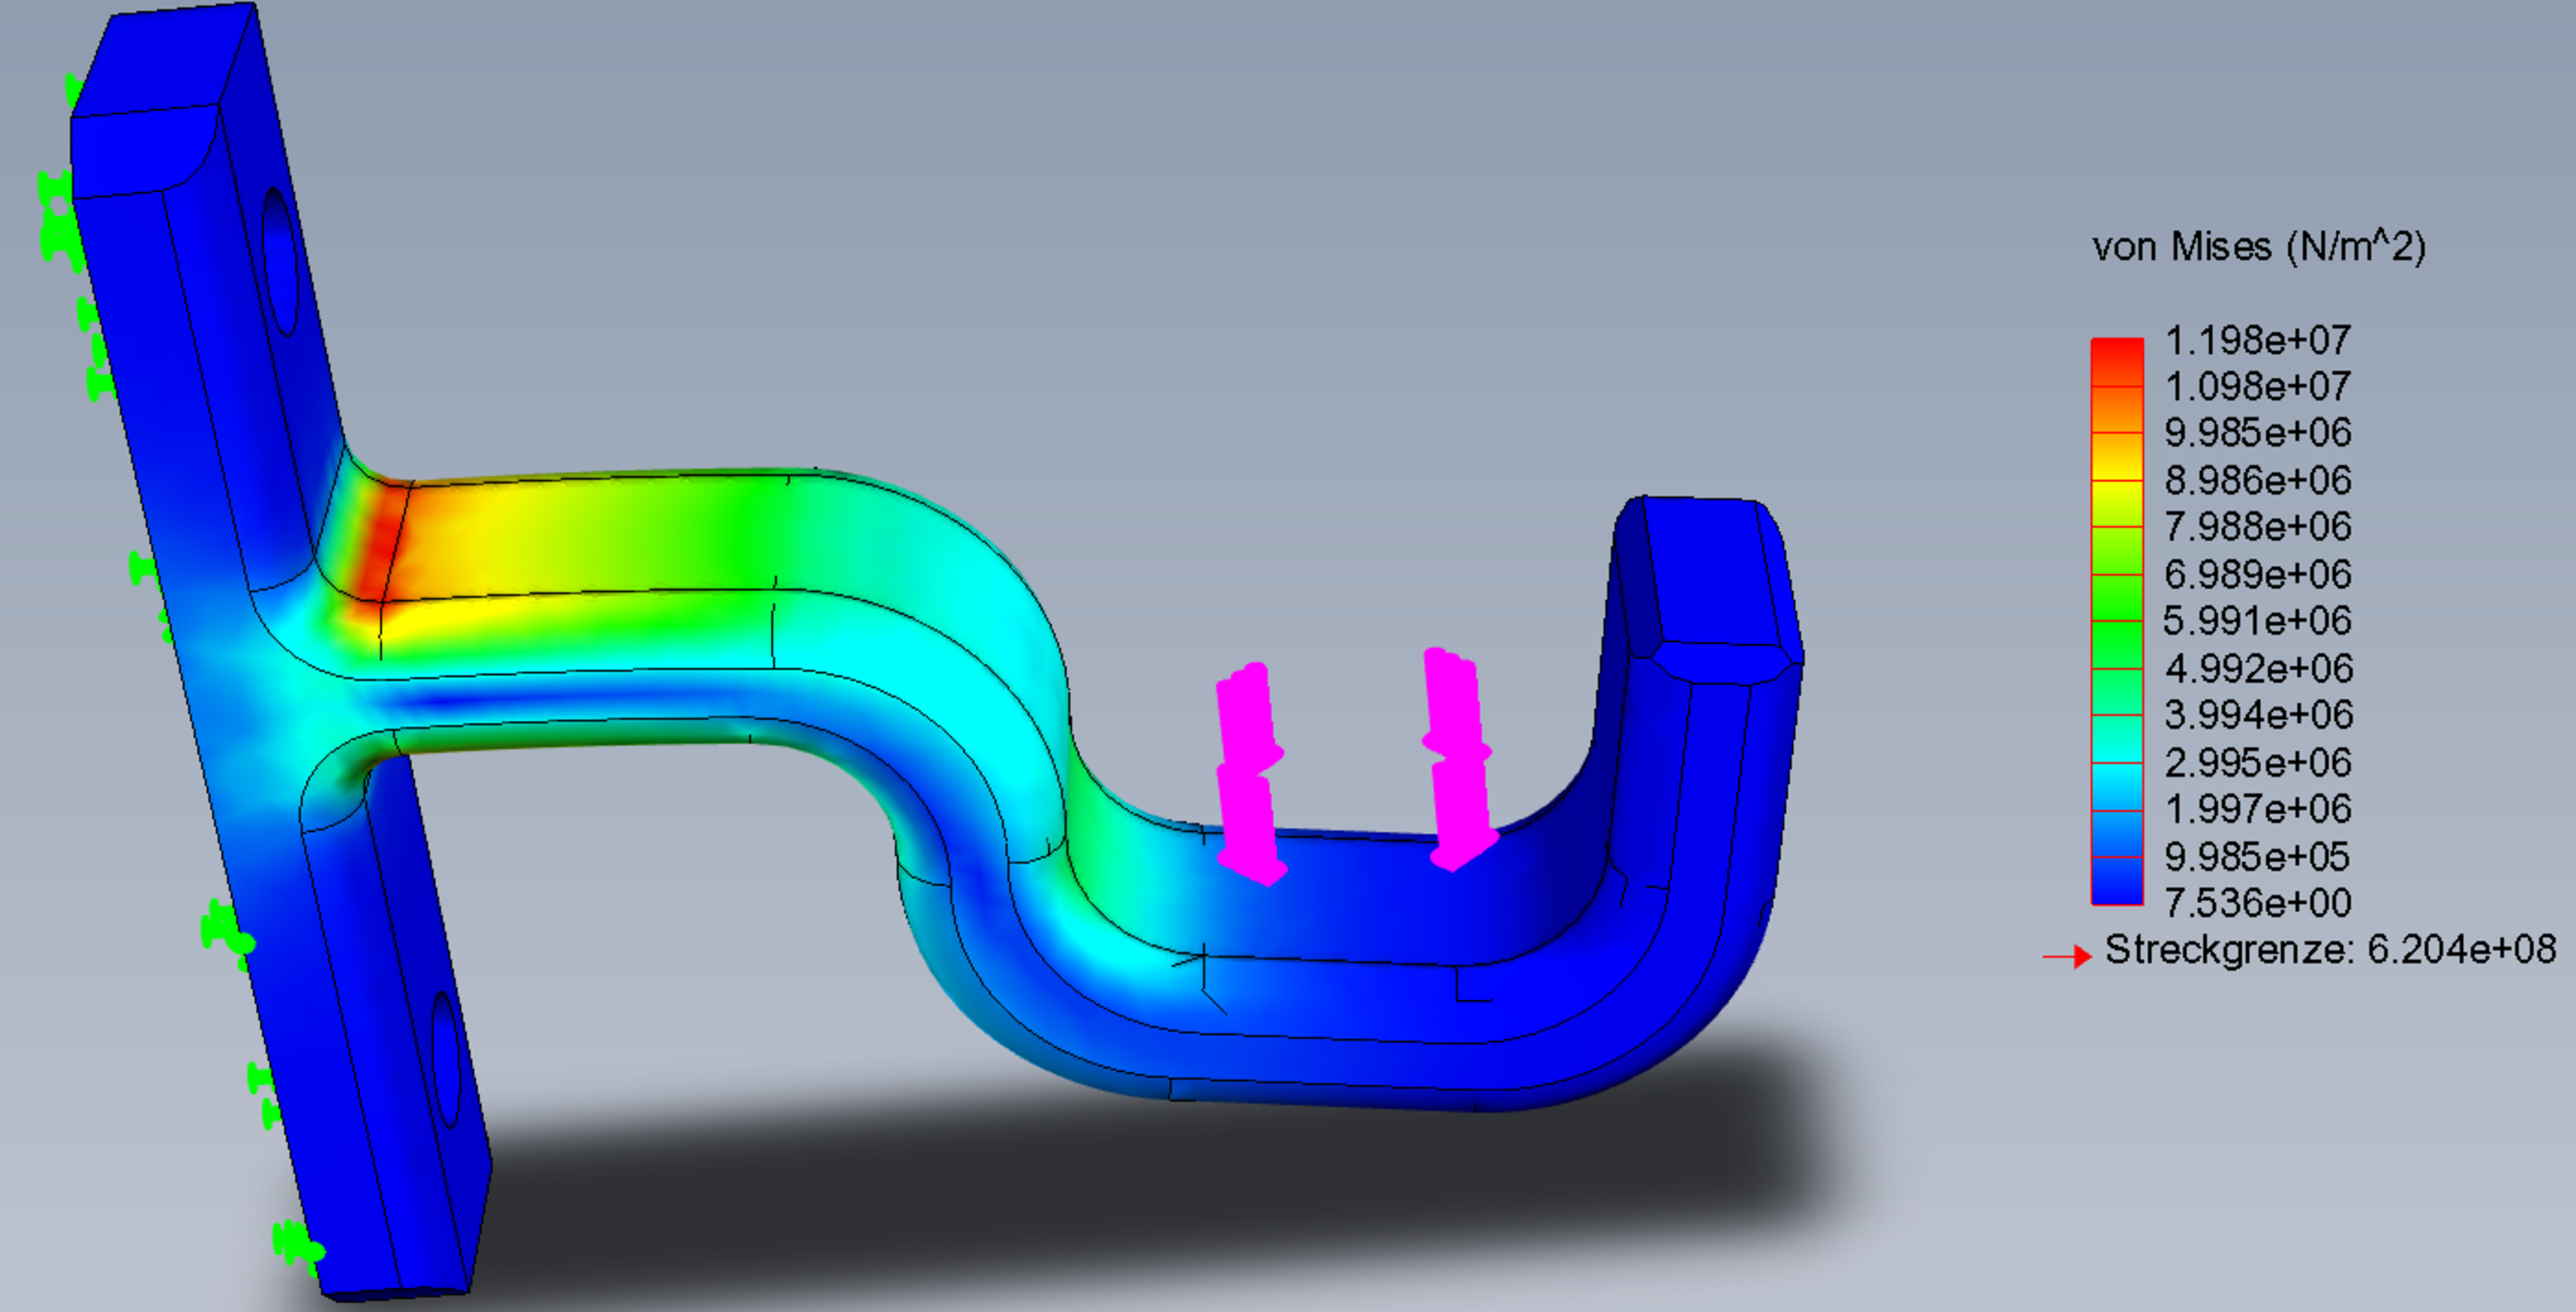
\includegraphics[width=0.8\textwidth]{chapter2/pictures/haken.pdf}
		    
		    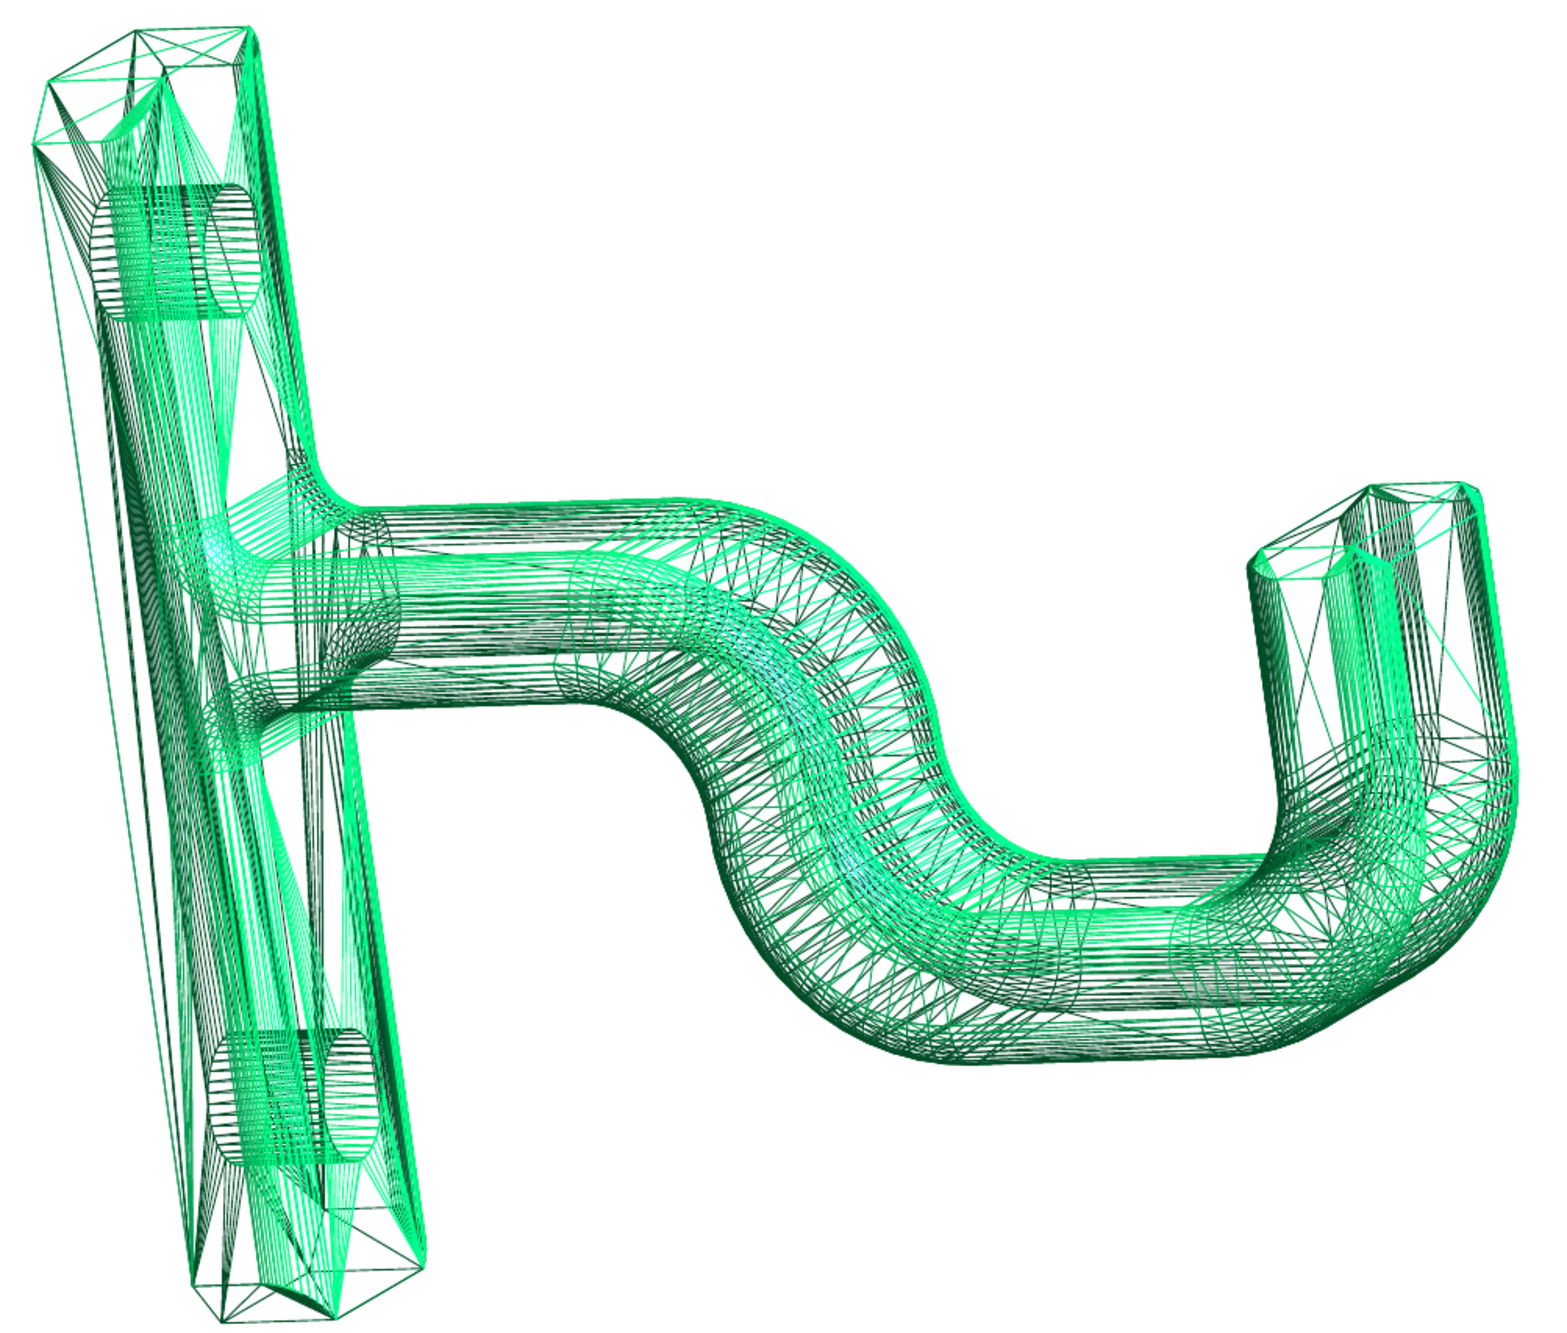
\includegraphics[width=0.6\textwidth]{chapter2/pictures/mesh.pdf}
		    \end{center}

		    \item \textbf{Tesla} wie Quadro, aber ohne Video-Controller. Diese sind im Wesentlichen für Deep-Learning Techniken gedacht. Moderne GPUs beinhalten sogenannte Tensorkerne, die für \textit{deep-convolutional neural networks} optimiert sind. Diese kommen nun vermehrt in Gaming Karten als Unterstützung für Ray-Tracing Kerne zum Einsatz.
		\end{itemize}		 		
		
        Karten aller drei Linien werden nach ihrer Chiparchitektur klassifiziert. Von der ältesten zur modernsten heißen diese: Tesla (nicht verwechseln!), Fermi, Maxwell, Kepler, Pascal, Volta (Weiterentwicklung: Turing)
        
        Zudem existieren Unterkategorien, die in der sogenannten \textit{\gls{compute capability}} zum Ausdruck kommen. Diese ist die wesentlichste Kenngröße einer Nvidia Grafikkarte, da sie bestimmt, welche Features von CUDA in Hardware auf der GPU implementiert sind.		
		
		Eine GPU ist im Wesentlichen ein Verbund aus tausenden Kernen, sogenannten \Glspl{Thread}, mit relativ geringer Leistung. Nach dem SIMD Prinzip führen alle Kerne ähnliche Tätigkeiten aus. Die Idee hinter HPC auf GPUs ist, die massive Parallelität für Tätigkeiten auszunutzen, die bestimmte Eigenschaften erfüllen:
		\begin{itemize}
			\item Probleme mit extrem hoher Parallelität, z.B. sehr große unabhängige Schleifen.
			\item Probleme mit sehr vielen ähnlich gelagerten Berechnungen, also die selben Operationen in der gleichen Reihenfolge aber mit unterschiedlichen Daten.
			\item Probleme mit einer geringen \Gls{Arbeit} in jedem parallelen Prozess, z.B. einfache mathematische Formeln.
			\item Probleme mit geringem Speicherfluss.			
		\end{itemize}

		Eine GPU wird aufgeteilt in eine bestimmte Anzahl von sogenannten Streaming Multiprocessors (\Gls{SM}). Üblich ist eine geringe zweistellige Anzahl (Abb. \ref{2:gpu}). Diese bestehen wiederum aus den folgenden Komponenten:
		
		\begin{itemize}
	        	\item Multiple Threaded Instruction Unit (\Gls{MTIU}): verteilt die Instruktionen auf einen \Gls{Thread} pro \Gls{Warp}
        		\item \Glspl{Warp}: ein Verbund von 32 \Glspl{Thread}. Eine Instruktion wird kopiert und an alle weitergegeben.
		    \item \Gls{Halfwarp}: Genau eine Hälfte eines \glspl{Warp}
		    \item Special Function Unit (SFU): Erledigt besondere Aufgaben, z.B. shader Berechnungen (später mehr) 
        		\item \Gls{shared Memory}: ein kleiner, extrem schneller Speicher, den sich alle \Glspl{Thread} eines \Gls{SM}s teilen.
		\end{itemize}
		
		\begin{figure}[h]
			\centering
    	        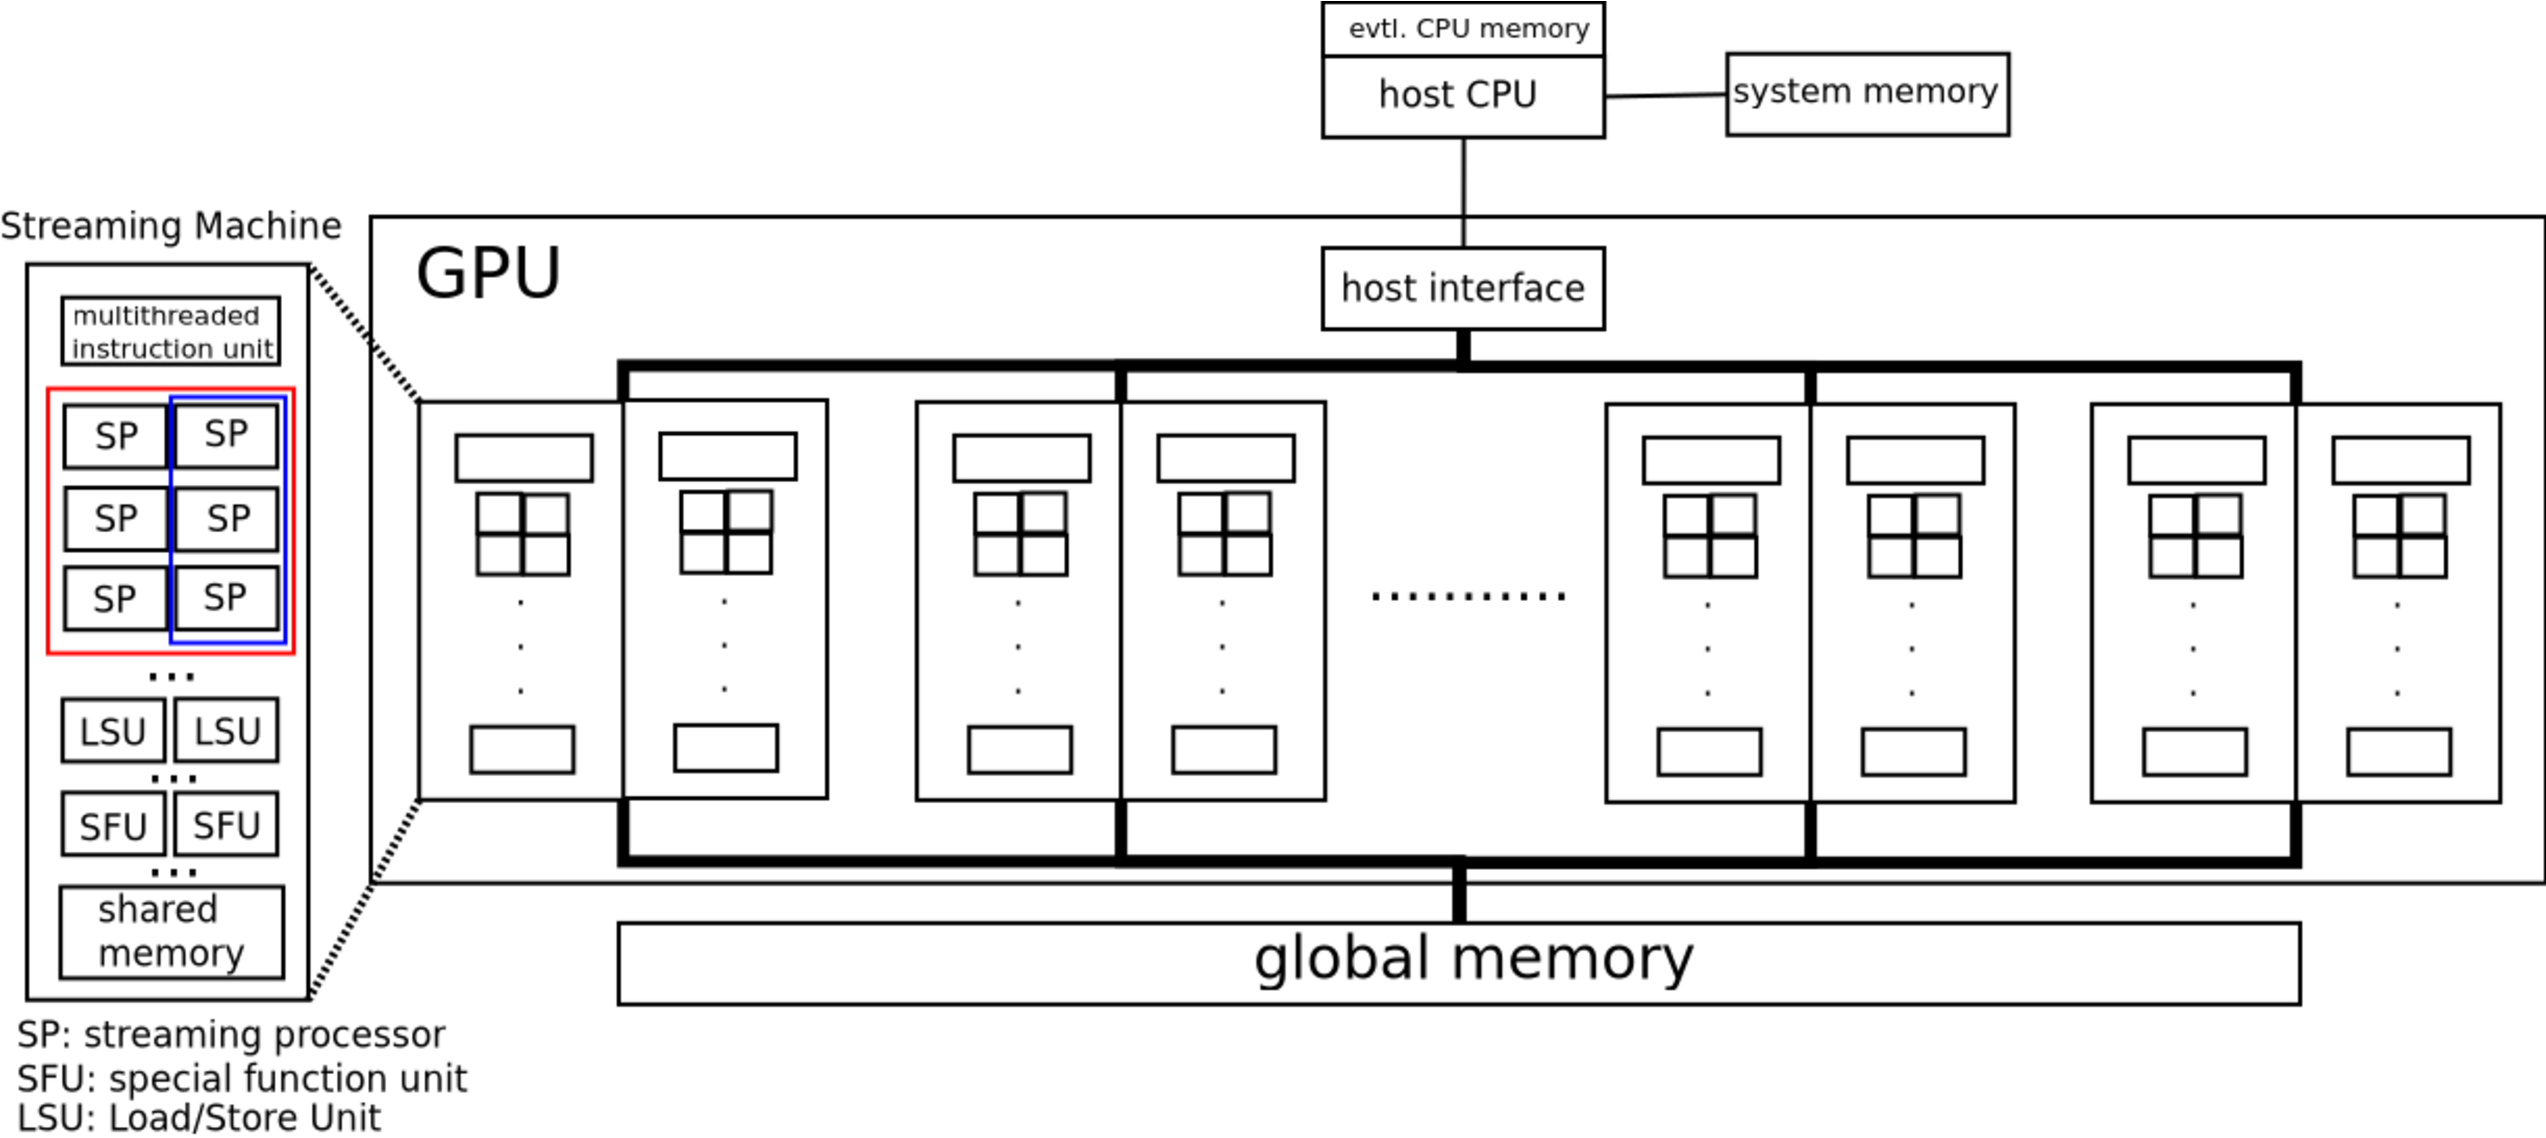
\includegraphics[width=\textwidth]{chapter2/pictures/sm.pdf}
    	        \caption[GPU]{Aufbau einer GPU}
    		    \label{2:gpu}
		\end{figure}

		Es ist wichtig, die technischen Details der Hardware zu kennen, um die Software darauf anzupassen. Ein HPC Programm ist üblicherweise genau auf die Hardware zugeschnitten, auf der das Programm laufen soll. Die Generalisierung eines Problems ist nicht trivial und manchmal sogar unmöglich oder nur unter starken \Gls{Performance}verlusten zu erreichen.	